\chapter[PROCESSAMENTO DE DADOS]{PROCESSAMENTO DE DADOS}
\label{chapter:data}

A grande quantidade de geradores e consumidores de dados relacionados a cidades
inteligentes trazem a necessidade de três características para as aplicações:
\textit{volume}, \textit{velocidade}, e \textit{varidade} \cite{alnuaimi2015}.
Uma forma de atingir estes pontos é através do uso de tecnologias de Big Data,
responsáveis por armazenar, processar e analisar os dados das aplicações de
cidades inteligentes \cite{alnuaimi2015}. Como relatado, o InterSCity carece de
um serviço de processamento de dados mais adequado, e, a partir dos estudos
feitos neste capítulo, decisões a respeito do novo serviço de processamento
serão tomadas.

Serão detalhadas duas arquiteturas, Lambda e Kappa, e levantadas tecnologias
a serem usadas que abrangem duas formas de processamento: \textit{batch} e
\textit{streaming}. No processamento \textit{batch}, os dados são utilizados
em conjunto, e armazenados de uma forma específica antes de serem escalonados
para serem processados \cite{zheng2015real}. No processamento
\textit{streaming}, por outro lado, os dados são processados conforme estão
disponíveis \cite{zheng2015real} permitindo consulta a informações com menor
latência. Adaptações nas arquiteturas serão feitas em relação ao apresentado na
literatura, com o propósito de ficarem mais adequadas ao contexto de cidades
inteligentes, e mais plausíveis para o estado atual do InterSCity.

\section{ARQUITETURA LAMBDA}

A Arquitetura Lambda é um padrão de projeto para plataformas de processamento
de dados que utilizam tecnologias Big Data \cite{kiran2015}, e surge como um
caminho alternativo a outras arquiteturas mais antigas, como a incremental com
\textit{sharding} \cite{marz2015}. É composta de três camadas: a camada
\textit{batch}\footnote{No decorrer do texto, as camadas da arquitetura Lambda
e outros termos associados não serão traduzidos.}, a camada \textit{serving}; e
a camada \textit{speed} \cite{kiran2015}. Cada uma destas camadas é
implementada utilizando algoritmos e ferramentas específicas, de modo
que certas ferramentas são mais apropriadas em certos contextos.

A \textbf{camada \textit{batch}} é responsável pelo processamento de uma grande
massa de dados, e tem como ponto fraco a alta latência. Em sua execução, ela
cria e gerencia um \textit{master dataset}\footnote{O \textit{master dataset} é um lote
histórico de informação, que, por ser imutável, só possibilita \textbf{anexação}
de informações.}, que, após processado, têm seus resultados condensados em
\textit{batch views}, utilizados pela \textbf{camada \textit{serving}}.
A camada \textit{batch} é então, em sua essência, imutável, de modo que, caso
uma mudança seja necessária, uma abordagem diferente deve ser seguida: o dado
que carece alteração não sofre transformações, permanecendo inalterado, mas um
novo dado com as alterações é inserido no lote \cite{marz2015}.

A \textbf{camada \textit{speed}} tem como diferencial o processamento com baixa
latência, que é obtido pelo uso de uma parcela menor da massa de dados\footnote{
A camada \textit{speed} só leva em conta dados que surgiram após a camada
\textit{batch} ter começado seu processamento.}. Outra característica importante
é que esta camada faz uso do processamento \textit{streaming}, que ocorre
quando os dados são processados conforme estão disponíveis. Este tipo de
processamento funciona bem com mecanismos de passagem de mensagem
\cite{marz2015}, e permitem que as consultas feitas levem em conta dados
recentes, ignorados pela camada \textit{batch}. Essa característica da
camada \textit{speed} também é conhecida como incremental, e costuma aceitar
também alteração de dados já utilizados e processados, tornando esta camada
mutável, o que força o uso de um banco de dados que suporte escrita aleatória,
aumentando substancialmente a complexidade desta camada \cite{marz2015}. Por
fim, a camada \textit{speed} condensa os resultados de seu processamento em
\textit{real-time views}, que serão fundidos com os resultados das
\textit{batch views} para que seja apresentado o resultado final. Os resultados
da camada \textit{speed} são então dispensados sempre que um \textit{batch}
terminar seu processamento \cite{marz2015}.

\begin{figure}
  \centering
    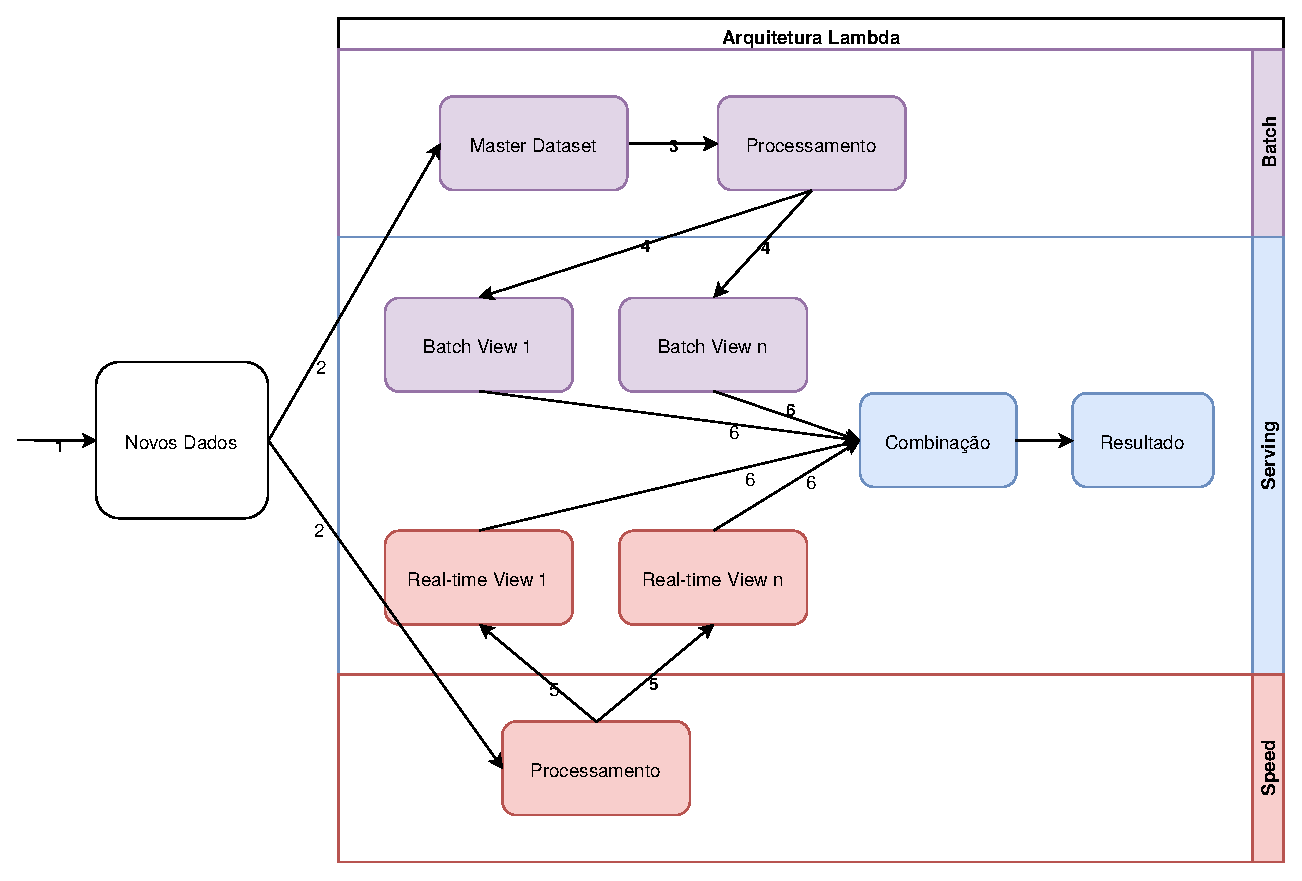
\includegraphics[width=\textwidth]{figuras/lambda-lifecycle.eps}
  \caption{Ciclo de vida na Arquitetura Lambda.}
  \label{fig:lambda-lifecycle}
\end{figure}

Um ciclo de vida típico da Arquitetura Lambda pode ser acompanhado na Figura
\ref{fig:lambda-lifecycle}, e tem seu início com a (1) chegada
de novos dados, que serão então (2) transmitidos tanto para a camada
\textit{batch} quanto para a camada \textit{speed}. A camada \textit{batch}
(3) anexa os novos dados, e os processa, (4) gerando assim
\textit{batch views}, que são enviados para a camada \textit{serving}. O mesmo
dado que foi enviado para a camada \textit{batch}, no passo (1), também foi
enviado para a camada \textit{speed}, onde (5) será processado com menor latência,
por só levar em conta dados recentes, gerando assim \textit{real-time views}. 
Caso uma consulta seja feita, ocorrerá então uma (6) soma entre os resultados
dos \textit{batch views} e \textit{real-time views}, que é então a resposta
a consulta \cite{marz2015}.

A Arquitetura Lambda garante sua resiliência através da \textit{isolação de
complexidade}, que é obtida graças a separação entre camadas \textit{batch}
e \textit{speed} \cite{marz2015}. A resiliência é obtida pois, uma vez que os
resultados são processados na camada \textit{batch}, os resultados da camada
\textit{speed} podem ser descartados. Essa técnica é essencial, já que o
processamento em tempo-real pode criar inconsistências, por conta da baixa
precisão que é ocasionada por usar somente dados recentes; contudo, essa
inconsistência é corrigida no próximo \textit{batch} a ser processado,
possibilitando que os resultados incoerentes da camada \textit{speed} sejam
descartados \cite{marz2015}.

Quanto à sua implementação no InterSCity, a Arquitetura Lambda pode precisar de
adaptações. Na literatura, a camada \textit{serving} é a responsável pela
junção entre o resultado do processamento feito pelas camadas \textit{speed} e
\textit{batch}, e a separação entre as camadas \textit{batch} e \textit{serving}
é bem definida \cite{marz2015}, contudo, isso depende das ferramentas que
serão definidas para uso. 

\section{ARQUITETURA KAPPA}

A Arquitetura Kappa é um padrão de projeto de \textit{software}, e surgiu após
questionamentos\footnote{\url{https://www.oreilly.com/ideas/questioning-the-lambda-architecture}}
quanto a complexidade da Arquitetura Lambda. É uma arquitetura recente (2014),
simples, e se baseia somente no uso da \textbf{camada \textit{speed}}
\cite{seyvet2016}. É guiada por quatro princípios:
(i) tudo é um \textit{stream}; (ii) os dados devem ser imutáveis; (iii)
somente um \textit{framework} para processamento deve ser utilizado; (iv) a
reprodução histórica deve ser disponível \cite{seyvet2016}.

Fazendo uso da observação de que o \textit{log} é um conjunto de informações
imutáveis e com ordenação bem definida, a Arquitetura Kappa o utiliza, e,
assim, atinge os quatro princípios citados anteriormente \cite{kreps2014}. O
\textit{log} é processado em tempo real, permitindo consultas em baixa
latência, com a possibilidade de acesso de dados atuais e históricos
\cite{forgeat2015}. Caso o processamento seja iniciado após o fluxo de dados já
ter começado, duas opções são possíveis: processar o \textit{log} do início,
tornando disponível os dados históricos, ou processar a partir do final,
não tendo acesso aos dados históricos, mas tendo latência mínima
\cite{kreps2014}.

\begin{figure}
  \centering
    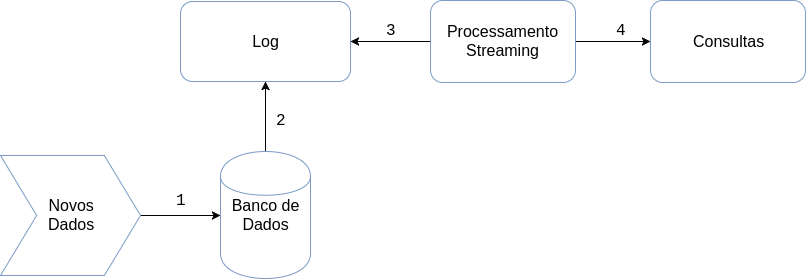
\includegraphics[scale=0.5]{figuras/kappa_architecture.png}
  \caption{Funcionamento da Arquitetura Kappa.}
  \label{fig:kappa-lifecycle}
\end{figure}

O funcionamento da Arquitetura Kappa está apresentado na Figura
\ref{fig:kappa-lifecycle}. Inicialmente, novos dados chegam à plataforma, e são
(i) persistidos no banco de dados, que (ii) anexa os resultados das transações
no \textit{log}. As mudanças no \textit{log} são observadas e
(iii) processadas pelo processamento \textit{streaming}, que, por fim, permite
a (iv) consulta do processamento feito.

Assim como levantado a respeito da Arquitetura Lambda, a implementação da
Arquitetura Kappa também precisaria de adaptações para ser implantada no
InterSCity, principalmente pelo uso do \textit{log}, que, dependendo das
tecnologias utilizadas, pode ser acessado de maneira mais ou menos conveniente.
Um casamento entre as tecnologias escolhidas deve ocorrer para que a
arquitetura seja implementada como sugerido na literatura, o que pode não ser
possível dadas as restrições da plataforma. O InterSCity no momento não
disponibiliza seus \textit{logs} de uma forma facilmente digeridas por
ferramentas usáveis na Arquitetura Kappa, forçando a busca por mais ferramentas,
ou até mesmo substituição quanto ao uso do \textit{log}.

\section{BROKER}

A comunicação entre diferentes módulos em plataformas de processamento de dados
pode se dar de diferentes modos, e um destes é através da passagem
de mensagem via PubSub, já utilizado pelo InterSCity \cite{delesposte2017}.
O \textbf{broker} é o mediador responsável por orquestrar as diferentes
mensagens que são transmitidas via PubSub \cite{marz2015}, e é primordial no
funcionamento das duas arquiteturas Big Data mencionadas anteriormente.

Uma abstração que facilita a compreensão do \textit{broker} é pensá-lo como o
mediador de um sistema de notícias. Uma entidade, desejando transmitir
uma notícia, a publica em um \textbf{tópico}, sendo então o produtor do
conteúdo. Outras entidades que desejam ser notificadas sobre aquele tema, se
inscrevem no tópico associado, e serão notificadas quando uma notícia referente
for publicada, sendo assim os consumidores do sistema. O \textit{broker} então
gerenciado esse processo, e tem a tarefa de transferir as mensagens de um
emissor para receptores, podendo ser, ainda, tolerante à falhas.

\begin{figure}
  \centering
    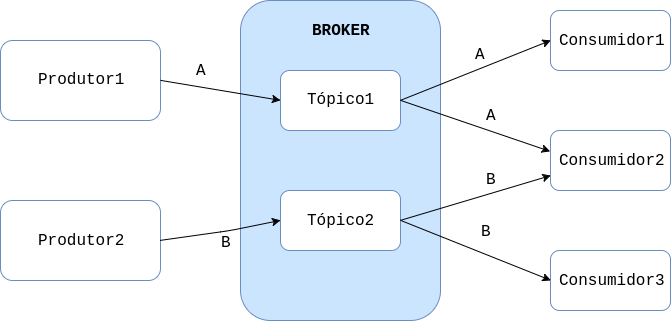
\includegraphics[scale=0.5]{figuras/broker.png}
    \caption{Funcionamento do \textit{broker}.}
  \label{fig:broker}
\end{figure}

A Figura \ref{fig:broker} ilustra o funcionamento do \textit{broker}, onde é
apresentado um cenário típico de atuação. No exemplo mostrado, a mensagem A
é transmitida pelo Produtor1 no Tópico1, e a mensagem B é transmitida pelo
Produtor2 no Tópico2. O Consumidor1 e o Consumidor2 recebem a mensagem A, por
estarem escritos no Tópico1, e os consumidores Consumidor2 e Consumidor3
recebem a mensagem B, por estarem registrados no Tópico2. Este funcionamento
pode receber variações, a depender das tecnologias utilizadas, e será útil
na implementação das arquiteturas Kappa e Lambda, sendo o
\textit{broker} o responsável por recuperar novas informações e as
disponibilizar para as ferramenta de processamento.

\section{COMPARATIVO ENTRE TECNOLOGIAS}

Nesta seção serão levantadas e comparadas alternativas para compor a
arquitetura do novo serviço de processamentos do InterSCity. As ferramentas
foram separadas nas categorias \textit{processamento batch},
\textit{processamento streaming}, e \textit{broker}. Ferramentas de banco de
dados não foram analisadas, pois uma troca seria prejudicial e não interessante
para a equipe do InterSCity. Um \textit{broker} diferente do utilizado pelo
InterSCity foi analisado considerando sua atuação somente com o serviço de
processamento, não alterando os microsserviços da plataforma.

\subsection{Ferramentas de Processamento Batch}

Duas ferramentas de processamento \textit{batch} foram analisadas: o
\textbf{Apache Hadoop MapReduce}, precursor no ecossistema Big Data, e o
\textbf{Apache Spark}, ferramenta mais recente. O MapReduce é uma das
ferramentas que compõe o ecossistema do Hadoop, e já foi utilizado em contextos
extremos\footnote{Lista das empresas que utilizam ou já
utilizaram o Hadoop: \url{https://wiki.apache.org/hadoop/PoweredBy}}, atuando
com excelência em cenários de grande massa de dados \cite{zaharia2008}, e sendo
assim uma escolha segura para compor a camada \textit{batch} da Arquitetura
Lambda. Só dispõe de API nativa para linguagem Java, de modo que a
implementação do MapReduce no InterSCity deva utilizar o uso da saída e entrada
padrão do sistema operacional, permitindo assim o uso da linguagem Ruby,
melhorando a adaptação da ferramenta pelo time do InterSCity.

Um dos questionamentos feitos ao MapReduce é em relação ao constante acesso e
uso do disco, que deve ser feito sempre que um \textit{job} é finalizado. Por
conta desta característica, seu uso não é facilmente justificável em cenários em
que a massa de dados não é grande o suficiente, e uma opção válida nestes casos
acaba sendo o Apache Spark, que evita o uso do disco através de
\textit{micro-batches} \cite{arsalan2014}. Estes \textit{micro-batches} têm seu
tempo de processamento definidos em código, de modo que seja possível definir
tempos de \textit{micro-batches} pequenos o suficiente para que seja considerado
tempo-real\footnote{O tempo-real mencionado durante este trabalho se refere ao
\textit{soft real-time}.}.

Outras características importantes do Spark para o contexto do
InterSCity são: API nativa em Python, Scala, Java, e R; biblioteca de
\textit{streaming}, permitindo que o Spark seja utilizado também na camada
\textit{speed} da Arquitetura Lambda; e biblioteca de clusterização e
aprendizagem de máquina, que pode ser útil para compor um futuro \textit{pipeline
de dados} do InterSCity. A Tabela \ref{tab:graysort2014results} apresenta
um comparativo entre performance do MapReduce e do Spark baseado em uma
competição que ocorreu em 2014, chamada
SortBenchmark\footnote{\url{http://sortbenchmark.org/}}. Na competição, o Spark
apresentou uma performance três vezes maior que o Hadoop MapReduce, utilizando
dez vezes menos recursos.


\begin{table}[!htbp]
    \centering
    \caption[Resultados da Sort Benchmark 2014, categoria GraySort]{Resultados da Sort Benchmark 2014, categoria GraySort. Fonte: Databricks, 2014\footnotemark.}
    \label{tab:graysort2014results}
    \resizebox{\textwidth}{!}{%
        \begin{tabular}{|l|l|l|l|}
            \hline
             & \textbf{Hadoop MRRecord}      & \textbf{SparkRecord}             & \textbf{Spark1 PB}               \\ \hline
             Data Size                    & 102.5 TB                      & 100 TB                           & 1000 TB                          \\ \hline
             Elapsed Time                 & 72 mins                       & 23 mins                          & 234 mins                         \\ \hline
             \# Nodes                     & 2100                          & 206                              & 190                              \\ \hline
             \# Cores                     & 50400 physical                & 6592 virtualized                 & 6080 virtualized                 \\ \hline
             Cluster disk throughput      & 3150 GB/s(est.)               & 618 GB/s                         & 570 GB/s                         \\ \hline
             Sort Benchmark Daytona Rules & Yes                           & Yes                              & No                               \\ \hline
             Network                      & dedicated data center, 10Gbps & virtualized (EC2) 10Gbps network & virtualized (EC2) 10Gbps network \\ \hline
             \textbf{Sort rate}           & \textbf{1.42 TB/min}          & \textbf{4.27 TB/min}             & \textbf{4.27 TB/min}             \\ \hline
             \textbf{Sort rate/node}      & \textbf{0.67 GB/min}          & \textbf{20.7 GB/min}             & \textbf{22.5 GB/min}             \\ \hline
        \end{tabular}
    }
\end{table}

\footnotetext{\url{https://databricks.com/blog/2014/11/05/spark-officially-sets-a-new-record-in-large-scale-sorting.html}}

\subsection{Ferramentas de Processamento Streaming}

Duas ferramentas de processamento \textit{streaming} foram analisadas: O
\textbf{Apache Storm}, escrito por Nathan Marz, criador da Arquitetura
Lambda, e o \textbf{Apache Spark}, analisado anteriormente como ferramenta de
processamento \textit{batch}. O Apache Storm permite o uso de qualquer
linguagem de programação que interaja com a saída e entrada padrão do sistema
operacional, e, sendo sugerido por Nathan Marz em seu livro sobre a Arquitetura
Lambda \cite{marz2015}, se faz uma opção segura para compor a camada
\textit{speed} da Arquitetura Lambda.

O Spark é utilizado como ferramenta de \textit{streaming} graças ao seu módulo
Spark Streaming, que tem nativamente integração com várias ferramentas que
podem servir de produtores, como o Kinesis, Kafka, HDFS, dentre outras. O
grande diferencial entre o Spark e o Storm é que o Spark faz processamento
\textit{streaming} via \textit{micro-batches}, ou seja, processa em intervalo
de tempos pré-definidos, enquanto o Storm processa em tempo-real, conforme
chegam novos dados. Essa diferença resulta em um tempo de latência notável
entre os dois, onde o Spark apresenta tempo de latência com pouca variância
conforme o volume de dados aumenta, enquanto o Storm apresenta latência mínima
com baixo volume de dados, mas que vai aumentando conforme o volume aumenta.
Um estudo feito relatou a diferença de performance entre as duas
ferramentas\footnote{\url{http://xinhstechblog.blogspot.com.br/2014/06/storm-vs-spark-streaming-side-by-side.html}},
contudo, foi feita com uma massa de dados pequena, sendo um cenário favorável
para o Storm.

O Storm então apresenta como vantagem em relação ao Spark a performance
superior e a flexibilidade de uso da linguagem Ruby, já utilizada pelo time
do InterSCity, porém, o Spark conta com a possibilidade de processamento
\textit{batch}, integração nativa com ferramentas produtoras, e o acesso a
ferramentas de clusterização e aprendizagem de máquina, que, por serem
interessantes para o InterSCity, equilibram o \textit{trade-off} entre as
duas ferramentas.

\subsection{Broker}

Dois \textit{brokers} foram analisados: o \textbf{RabbitMQ},  utilizado
extensivamente pelo InterSCity, e o \textbf{Apache Kafka}, constantemente
referenciado para implantação da Arquitetura Kappa. O RabbitMQ é um
\textit{broker} bem difundido, utilizado por empresas como a Cisco, Instagram,
New York Times, dentre outros \footnote{\url{https://www.rabbitmq.com/}},
e apresenta suporte para diversas linguagens \cite{zaitsev2014}, o que
facilitou sua adoção pelo time do InterSCity. Entre seus diferencias em relação
a outros \textit{brokers}, podem ser destacados: tolerância a falhas,
processamento distribuído, alto desempenho, filas (e tópicos) com composições
mais complexas, e a possibilidade de uso de
\textit{plugins}\footnote{\url{https://www.rabbitmq.com/plugins.html}},
que suportam, por exemplo,
federação\footnote{\url{https://www.rabbitmq.com/federation.html}}.

O Apache Kafka, embora seja uma ferramenta mais nova\footnote{O RabbitMQ teve
sua primeira \textit{release} em 2007, e o Apache Kafka em 2011.}, também é
utilizado em contextos extremos por várias
empresas\footnote{\url{https://cwiki.apache.org/confluence/display/KAFKA/Powered+By}}.
Tendo como um dos principais diferenciais a performance e escalabilidade,
recentemente foi capaz de lidar com mais de 1.4 trilhões de mensagens diárias,
distribuídas sobre 1400 nós \cite{koshy2016}. Um outro diferencial relevante
entre o Kafka e os outros concorrentes é o suporte padrão à integração entre
\textit{logs} e tópicos, vital na implementação da Arquitetura Kappa. Ainda,
o Kafka conta com sistema de tolerância a falhas e suporte a várias linguagens de
programação\footnote{\url{https://cwiki.apache.org/confluence/display/KAFKA/Clients}}.

Ambas as opções são então sólidas e adequadas para o uso do InterSCity. A
performance entre os dois já foi comparada, e, embora o Kafka tenha tido
performance
superior\footnote{\url{http://www.cloudhack.in/2016/02/29/apache-kafka-vs-rabbitmq/}},
a performance do RabbitMQ não compromete o uso no InterSCity. Assim, os pontos
cruciais na escolha de tecnologia devem ser: o fato do Kafka ter suporte a
\textit{log} e \textit{handler} nativo para o Spark, e o RabbitMQ já sendo
utilizado pelo InterSCity e possibilitando o uso de \textit{plugins}, como de
\textit{web-socket}.

